\thispagestyle{plain}
\begin{center}
    \Large
    \textbf{Journal: Computational Intelligence and Neuroscience}
    \vspace{0.4cm}
    
    \textbf{Self Sovereign Identity Approach in oAuth 2.0}
    \vspace{0.4cm}
    \large
    
    %Thesis Subtitle
    \vspace{0.4cm}
    
    \textbf{Dr.Shailesh Kumar, Dr. Prashant. B. Kumbharkar, and Sujeet Suryawanshi}
       
    \vspace{0.9cm}
    %manage the history of their activity and the contents that they created and shared with other users.
\end{center}
\section*{Abstract}

Identity management, encompassing authentication and authorization within a networked environment, stands as a paramount security aspect. Over time, various identity management paradigms have evolved, progressing from the isolated silo model to the federated model and, more recently, the self-sovereign identity (SSI) approacg. Notably, SSI empowers users to autonomously oversee their own data, irrespective of organizational involvement, through the utilization of emerging blockchain technology. Numerous ongoing studies are exploring the potential of SSI.

Nevertheless, SSI adoption has remained limited due to its inherent compatibility issues and user inconveniences, stemming from an unfamiliar user experience and a nascent development phase. In response, this research paper proposes a novel SSI approach rooted in blockchain technology that aligns with the widely accepted and mature OAuth 2.0 standard. This blockchain-based model ensures users' data sovereignty, allowing them to wield control over their information in a decentralized manner, free from reliance on specific monopolistic service providers.

The proposed model boasts high usability and scalability, as it can be readily embraced and implemented by users and clients familiar with existing OAuth protocols. The feasibility of the proposed model is confirmed through its implementation, accompanied by a thorough security analysis. It is anticipated that this innovative model will play a pivotal role in advancing both blockchain technology and the adoption of self-sovereign identity solutions.

\vspace{0.5cm}
\textbf{Keywords:} Self Sovereign Identity, Identity Management, OAuth

\section*{Introduction}


In the realm of internet-based identity management, models for user authentication and authorization have continuously evolved to address the shortcomings of previous approaches. In the initial identity approach, individual service providers held user information and directly carried out user authentication. However, the identity approach had limitations, primarily because authentication could only be conducted by the service provider that possessed the user data. This limitation subsequently resulted in the issue of password fatigue among users as the diversity of internet services expanded.

In order to address the shortcomings of the identity approach, the federated model was introduced. This approach aimed to resolve the issue by delegating authentication to a specific service. The federated approach was implemented in multiple variations.One of these variations was the single sign on, in which the delegated authentication server handles all authentication tasks within a single network, employing the SAML (Security Assertion Markup Language) protocol.Another approach involved OAuth, in which various third-party services delegated the responsibility of authentication and authorization to a specific service, such as Github, Apple ID,  utilizing the HTTP protocol. While the federated model successfully alleviated password weariness or exhaustion that users experience due to the repeated need to remember and manage multiple passwords for various online services, it introduced new challenges. The authentication service ended up accumulating vast quantities of user data, giving rise to both management and security concerns. Such a scenario raised the potential for privacy violations as the service could potentially misuse the user data it had accumulated. Additionally, a significant issue emerged where third-party services could experience disruptions in functionality if the authentication service experienced temporary failures or faced permanent suspension.
\par
The user-centric model emerged as a solution to provide users with greater control over their data and to address the issues encountered in previous models. An example of such a service was OpenID , but its widespread adoption faltered due to the unfamiliarity of its authentication process. Subsequently, several authentication services with similarities to OpenID were developed. However, many of these services closely resembled the federated model, lacking significant public appeal. Their susceptibility to phishing attacks further limited their adoption.
\par
The emergence of blockchain technology paved the way for the self-sovereign identity (SSI) approach, which effectively addressed the existing limitations while pursuing the same objectives as the user-centric approach. Blockchain's transparent and consistent nature helped resolve the data reliability issues associated with the earlier OpenID. Notable examples of blockchain-based SSI models include Veres One distributed ledger and IDunion network. Standardization efforts for the SSI approach are underway, with discussions on decentralized identifiers (DID) taking place within the World Wide Web Consortium (W3C).
\par
Nonetheless, numerous challenges remain to facilitate the widespread adoption of the SSI approach. Each SSI approach employs its unique authentication and authorization process, necessitating users to learn a new set of procedures for each model. Additionally, service developers face the burden of separately implementing this process for each SSI approach to integrate their services with them. While SSI approach have attempted to mitigate these issues through tutorial pages to aid user understanding and by offering development libraries for easier integration, these measures do not fundamentally resolve the aforementioned challenges.
\par
This research paper introduces an innovative open network-based self-sovereign identity (SSI) approach that effectively addresses the challenges outlined. The proposed model adheres to the core principles of the SSI model while also aligning with the well-established OAuth 2.0 framework, known for its maturity and widespread adoption. This integration with OAuth 2.0 simplifies both the development process and user experience, as users are already familiar with OAuth.
\par
In the proposed model, the principles of user-centric authentication and authorization are upheld through a design that empowers each user to assume the role of an authorization server within OAuth, utilizing their own device. Users can securely manage their information while offering a decentralized authentication and authorization process that is not reliant on a specific service provider, such as Github.
\par
The proposed model has the following contributions. First, it proposes SSI approach that complies with OAuth 2.0 standard, which results in high reliability and interoperability. Second, it provides novel user-centric authentication and authorization which are controlled under a user’s own device with the help of open network. Third, from the viewpoint of service developers, the proposed model can be easily applied to their service because it follows the flow of OAuth 2.0. Fourth, it enables a user to manage personal information in a both secure and high accessible way by storing the information in his own private device after encryption.
The rest of this paper presents the following. Section 2 shows how OAuth 2.0 works and it examines existing studies related to SSI. Section 3 describes the structure and processes of the proposed model. Section 4 displays the results of implementing the proposed model. Section 5 provides the results of a security analysis and Section 6 contains conclusions.

\section*{oAuth}

\subsection*{In brief}
The OAuth 2.0 authorization framework facilitates a third-party application in acquiring restricted access to an HTTP service in one of two ways. It can do so by coordinating an approval process between the resource owner and the HTTP service, effectively acting on behalf of the resource owner. Alternatively, the framework allows the third-party application to independently obtain access in its own right.
\subsection*{What is solves}
In the traditional client-server authentication model, when a client seeks access to a secured resource (known as a protected resource) on the server, it does so by verifying its identity with the server, utilizing the resource owner's credentials. To enable third-party applications to access these protected resources, the resource owner must disclose their credentials to these third parties. However, this approach presents several problems and limitations:
\begin{enumerate}

\item Credential Storage: Third-party applications are obligated to retain the resource owner's credentials for future use, typically storing the password in plaintext.

\item Password Dependency: Servers must support password-based authentication, even though passwords have inherent security weaknesses.

\item Broad Access: Third-party applications often acquire overly extensive access to the resource owner's protected resources, leaving resource owners without the ability to limit access duration or restrict access to specific subsets of resources.

\item Revocation Challenges: Resource owners are unable to revoke access for a specific third party without revoking access for all third parties, and they can only do so by changing the third party's password.

\item Compromised third party application: When a third-party application is compromised, it poses a significant security risk, as such a compromise can lead to the exposure of the end-user's password. Consequently, this breach could potentially grant unauthorized access to all data that is protected by that password. This underscores the importance of robust security measures and safeguards to prevent such compromises and protect user data.

\end{enumerate}
These issues underline the need for more secure and flexible authentication and authorization mechanisms, which OAuth 2.0 aims to address.
\par

OAuth effectively tackles these issues by introducing an authorization layer and separating the roles of the client and the resource owner. In OAuth, the client requests access to resources controlled by the resource owner and hosted by the resource server. Instead of utilizing the resource owner's credentials to access these protected resources, the client obtains an access token—a string that represents a specific scope, lifetime, and other access attributes. These access tokens are issued to third-party clients by an authorization server with the resource owner's approval. The client then employs this access token to access the protected resources hosted by the resource server.
\par
For instance, consider an end-user (resource owner) who wishes to grant a printing service (client) access to her protected photos stored on a photo-sharing service (resource server). Rather than sharing her username and password with the printing service, the end-user authenticates directly with a server trusted by the photo-sharing service (authorization server). This trusted server then issues delegation-specific credentials (access token) to the printing service, allowing it to access the specified resources without the need for the resource owner's sensitive login information.
\par
\par
\begin{figure}
        
        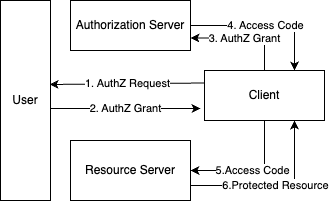
\includegraphics[width=8cm]{images/oauth.drawio.png}
        \centering
        \caption{oAuth2.0 in Brief}
        \label{fig:my_label}
    \end{figure}
A typical proposed flow for oAuth2.0 is as follows:
\begin{enumerate}
\item User (Resource Owner) connects with client and provides information on Authorization server it wishes to use to provide the required information (Protected resource)

\item Client requests for Authorization (AuthZ) to user
\item User provides information
\item Based on user provided information, Authorization Server checks if user is legitimate one and provides an 'Access code' that can be used by client for accessing the protected resource
\item Client uses 'Access Code' and communicates with resource server. Resource server verifies the 'Access Code' and provides protected resource to client.

\end{enumerate}
\section*{Self Sovereign Identity}
\subsection*{In brief}
Self-sovereign identity (SSI) offers the potential to establish a level of trust and autonomy in sharing or disseminating identity attributes in the digital realm that mirrors the control individuals have in the physical world. SSI adopts a user-centric approach, wherein the user maintains ownership of their data and isn't reliant on a central authority to verify their identity.
\par
In an SSI framework, users exercise complete authority over the information they choose to disclose and to whom they reveal it. Through a shared identity metasystem, users can verify their digital identity across diverse platforms and in various locations. Consequently, self-sovereign identity is characterized by privacy, security, and portability, delivering greater control and assurance in the digital realm.
\par
SSI implementations depart from hierarchical certification schemas and instead operate on the basis of a peer-to-peer and distributed "web of trust," devoid of root or intermediate Certificate Authorities (CAs).
\par
While there is an ongoing effort to establish the adoption of existing vendor-independent Self-Sovereign Identity (SSI) standards in the enterprise world and on the public internet, the integration of SSI into enterprise environments and landscapes is still a work in progress and lacks standardized practices.

In enterprise settings, where some services and applications are contained within a enterprises's internal infrastructure, delegated authentication is frequently implemented using company-owned identity providers, such as Active Directory or RedHat Keycloak. These company-owned Single Sign-On (SSO) solutions often extend to both web applications and "traditional" rich client applications. They utilize various protocols, including SAML, Kerberos, OAuth, and OIDC, to facilitate secure and streamlined authentication processes. However, achieving seamless integration of SSI into such enterprise environments remains a complex and evolving endeavor.

SSI systems offer enhanced privacy features, vulnerabilities such as identity spoofing and data breaches remain concerns. Exploring cryptographic techniques, zero-knowledge proofs, and robust authentication mechanisms can contribute to mitigating these risks \cite{503}.
\subsection*{What it solves}
\begin{figure}
        
        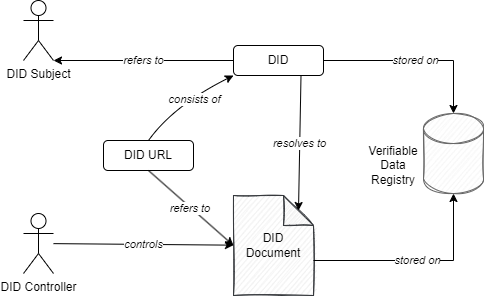
\includegraphics[width=10cm]{images/DID-Architecture.png}
        \centering
        \caption{SSI in Brief}
        \label{fig:my_label}
    \end{figure}
\subsubsection{DID Subject}
DID Subject can be an individual or a organisation or concept or a thing.
\subsubsection{DID Controller}
DID Controller can be a human or non-human.
\subsubsection{DID}
DID consists of scheme, DID-Method and DID-Method specific identifier. It refers to a DID subject. It resolves to a DID Document. It is stored on verifiable data registry.
\subsubsection{DID URL}
DID URL consists of DID and additional path to resource. Resource could be public key mentioned in DID document or it could also be external resource.
\subsubsection{DID Document}
DID Document contains information pertaining to cryptography proofs that can be used by controller to prove its control and additional information pertaining to DID methods and services relevant for interaction with DID subject.
\subsubsection{Verifiable Data Registry}
Its a system that facilitates storage of DIDs and DID documents and retrieval of same.
\subsubsection{DID Methods}
Mechanism to create, resolve, update and deactivate DID and respective DID document 
\subsubsection{DID resolver and DID resolution}
It accepts DID as input and produces a conforming DID document as output. This process is called DID resolution. The steps are defined by DID method specification for resolving a specific type of DID. 










    
\section*{Digital Identity Vault}


\begin{figure}
        
        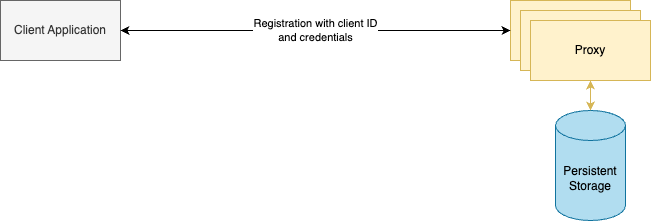
\includegraphics[width=15cm]{images/Client App Registration.drawio.png}
        \centering
        \caption{Client App Registration}
        \label{fig:my_label}
    \end{figure}


    \begin{figure}
        
        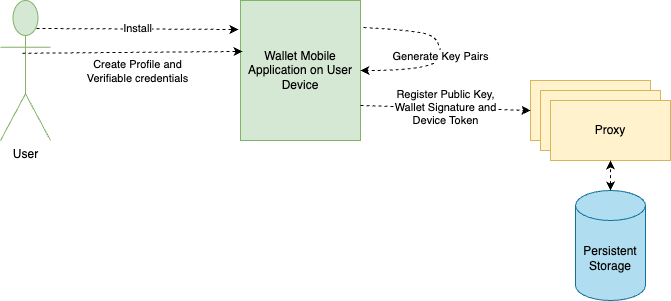
\includegraphics[width=15cm]{images/WalletRegistration.drawio.png}
        \centering
        \caption{Wallet registration}
        \label{fig:my_label}
    \end{figure}
    \begin{figure}
        
        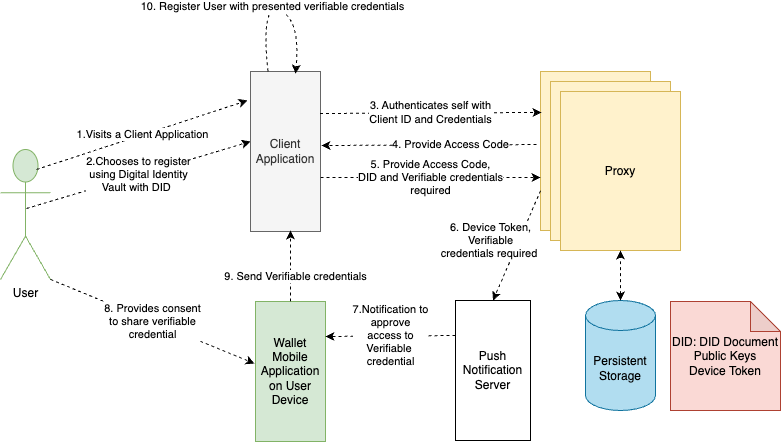
\includegraphics[width=15cm]{images/User Registration.drawio.png}
        \centering
        \caption{User Registration}
        \label{fig:my_label}
    \end{figure}
    \begin{figure}
        
        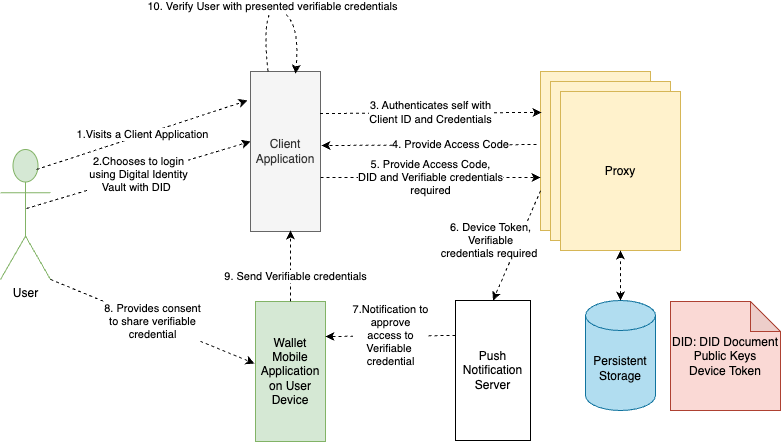
\includegraphics[width=15cm]{images/UserWalletClientAppLogin.drawio.png}
        \centering
        \caption{User Login}
        \label{fig:my_label}
    \end{figure}
Despite the development and proposal of Self-Sovereign Identity (SSI) models leveraging blockchain technology, widespread adoption has remained elusive. The core issue lies in the fact that each of these models adopts its distinct authentication and authorization process. This diversity in processes presents technical challenges when existing systems attempt to integrate the SSI model. Users are confronted with unfamiliarity and inconvenience when navigating these novel processes. Additionally, the security of these unique authentication and authorization methods has not undergone thorough analysis.
\par
In response to these challenges, this research paper introduces a novel SSI approach, which aims to address these fundamental issues.The presented approach aligns with the widely adopted OAuth framework, ensuring users have a familiar and comfortable experience through innovative authentication and authorization procedures based on OAuth principles. Leveraging open source and network technology, this model delivers decentralization and data integrity for both users and clients, thus ensuring the reliability of authentication and authorization processes. 
\par
This approach not only resolves the issues of information centralization and privacy concerns associated with existing federated identity management models controlled by major corporations but also empowers users with secure access to and control over their personal information, promoting data sovereignty.



\section*{Regulatory and Legal Challenges}
\subsection*{Digital Identity Legislation} 
The legal landscape surrounding digital identity and SSI is often complex and lacks uniformity. Researchers can delve into the development of harmonized legal frameworks that support SSI implementation across jurisdictions, while safeguarding individuals' rights and ensuring compliance with data protection regulations \cite{504}.
\subsection*{Liability and Accountability} Determining liability and accountability in SSI systems poses challenges, particularly in cases of identity-related fraud or errors. Investigating liability models and dispute resolution mechanisms within decentralized identity ecosystems is an area of potential research \cite{505}.

\section*{Societal and Adoption Challenges}
\subsection*{User Education and Acceptance}Achieving widespread adoption of SSI requires users to understand its benefits and functionalities. Research can focus on designing effective educational campaigns and user-friendly interfaces that encourage user acceptance and trust in SSI systems \cite{506}.
\subsection*{Inclusivity} Ensuring that SSI systems are accessible to all individuals, including marginalized communities, is crucial. Exploring ways to bridge the digital divide and address potential biases within SSI implementations is an avenue for further investigation \cite{507}.

\section*{Research Opportunities}
\subsection*{Usability and User Experience} Investigating ways to enhance the usability and user experience of SSI systems can drive greater adoption. This includes research on intuitive user interfaces, seamless integration with existing services, and minimizing user friction \cite{508}.
\subsection*{Decentralized Identity Ecosystems} Exploring the evolution of decentralized identity ecosystems beyond SSI presents intriguing research opportunities. This could involve the integration of blockchain technology, distributed ledger systems, and decentralized identifiers (DIDs) for broader applications \cite{509}.
\subsection*{Interdisciplinary Collaborations} Collaborative research efforts between computer scientists, legal experts, policymakers, and sociologists can yield comprehensive insights into the multifaceted challenges of SSI and guide its development in a holistic manner \cite{510}.

\section*{Conclusion}
Self-sovereign identity holds great promise as a transformative solution in the realm of digital identity management. However, the journey toward its widespread adoption is riddled with challenges that demand careful consideration and innovative research solutions. By addressing the technical, regulatory, and societal aspects outlined in this journal, the research community can pave the way for a future where individuals have greater control and agency over their digital identities.




